\chapter{Android 4 – Kommunikation \& Nebenläufigkeit}

\section{Netzwerk-Kommunikation (Communication)}

\subsection{Kommunikation über HTTP (zustandslos)}

HTTP (Hyper-Text Transfer Protokoll) ist ein zustandsloses Kommunikationsprotokoll welches über TCP/IP transportiert wird. Eine HTTP-Anfrage besteht aus einem Header und einem Body. Im Header befinden sich die Metadaten (z.B. Content-Length) und im Body der eigentliche Inhalt (Text, Bild usw.). Mit jeder Antwort liefert der Server einen Statuscode (z.B. 200 = OK).
Abbildung \ref{fig:http-anfrage} zeigt zwei unterschiedliche Möglichkeiten eine Anfrage an einen HTTP-Server unter Android zu senden. Der \texttt{HttpClient} ist zu bevorzugen. Für den Internet-Zugriff muss eine Berechtigung im Manifest eingetragen werden.

\begin{figure}
	\centering
	\begin{subfigure}[b]{0.4\textwidth}
		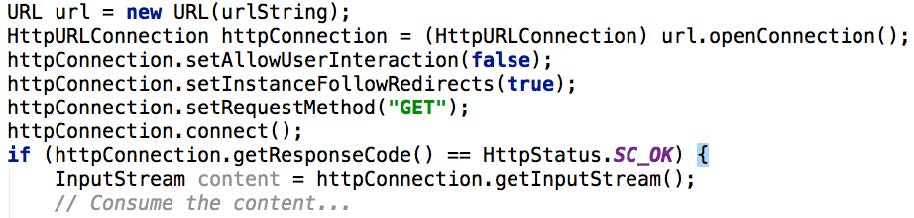
\includegraphics[width=\textwidth]{fig/httpurlconnection}
		\caption{\texttt{java.net.HttpURLConnection}}
	\end{subfigure}
	~
	\begin{subfigure}[b]{0.4\textwidth}
		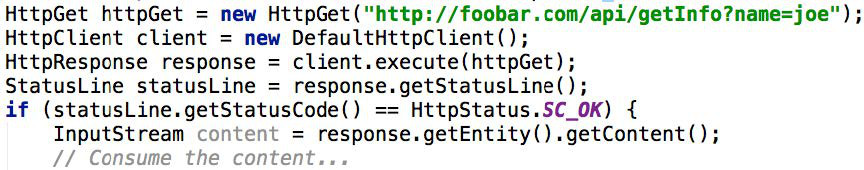
\includegraphics[width=\textwidth]{fig/httpclient}
		\caption{\texttt{org.apache.http.client.HttpClient}}
	\end{subfigure}
	\caption{Anfrage an HTTP-Server}
	\label{fig:http-anfrage}
\end{figure}

Beide Klassen liefern einen \texttt{InputStream} zurück. Dieser kann mit einem \texttt{BufferedReader} zeilenweise ausgelesen werden. Mit der statischen Methode \texttt{BitMapFactory.decodeStream(in)} können die Bytes von verschiedenen Bildertypen (JPG, PNG, GIF) in ein \texttt{Bitmap}-Objekt. Dieses kann dann auf einer beliebigen \texttt{ImageView} als Input gesetzt werden.

Daten von Webservices werden oft im JSON oder im XML Format ausgeliefert. JSON besteht aus Arrays und Objekten. Ein Array ist eine Sequenz von Elementen (\texttt{[]}). Ein Objekt ist ein Schlüssel-Werte-Paar (\texttt{{}}). Diese Elemente können beliebig geschachtelt werden. Abbildung \ref{fig:json} zeigt wie JSON geparst wird.

\begin{figure}
	\centering
	\begin{subfigure}[b]{0.4\textwidth}
		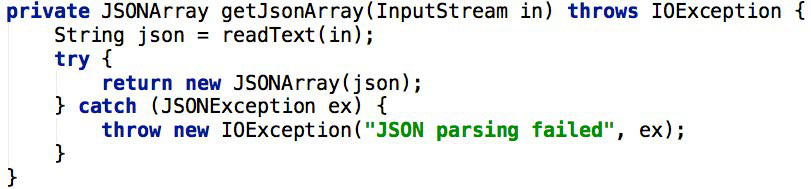
\includegraphics[width=\textwidth]{fig/json-array-erstellen}
		\caption{JSON-Array erstellen}
	\end{subfigure}
	~
	\begin{subfigure}[b]{0.4\textwidth}
		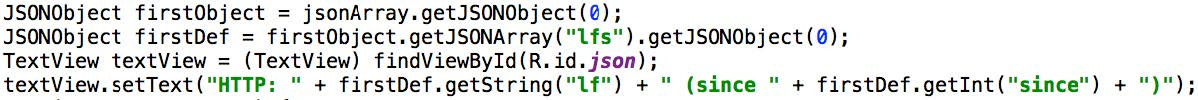
\includegraphics[width=\textwidth]{fig/json-array-auslesen}
		\caption{JSON-Array auslesen}
	\end{subfigure}
	\caption{JSON-Parsing}
	\label{fig:json}
\end{figure}

XML besteht aus Elementen (\texttt{<>}) welche Attribute besitzen können. Bei XML kann auch eine Vorlage definiert werden. Damit lässt sich XML besser validieren als JSON. Abbildung \ref{fig:xml} zeigt wie XML geparst wird.

\begin{figure}
	\centering
	\begin{subfigure}[b]{0.4\textwidth}
		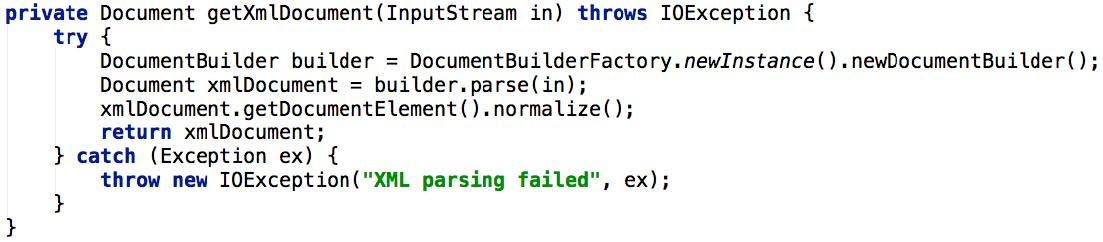
\includegraphics[width=\textwidth]{fig/xml-document-erstellen}
		\caption{XML-Document erstellen}
	\end{subfigure}
	~
	\begin{subfigure}[b]{0.4\textwidth}
		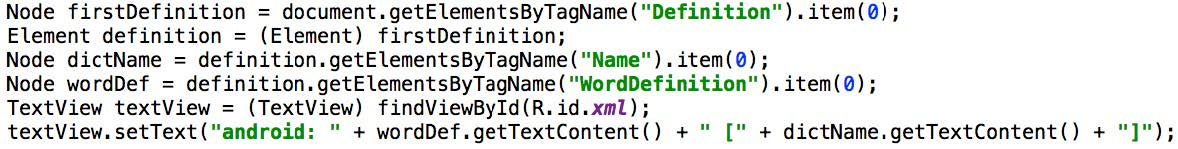
\includegraphics[width=\textwidth]{fig/xml-document-auslesen}
		\caption{XML-Document auslesen}
	\end{subfigure}
	\caption{XML-Parsing}
	\label{fig:xml}
\end{figure}

\subsection{Kommunikation über Sockets (zustandsbehaftet)}

Die Kommunikation über Sockets ist zustandsbehaftet und basiert auf TCP/IP. Für die Socketkommunikation existiert kein Protokoll (Sache der Teilnehmer). Deshalb wird über Datenströme bidirektional kommuniziert. Die Verbindung zwischen Client und Server bleibt bestehend. Dadurch ist es möglich dass der Server Push-Nachrichten an die Clients senden kann. Diese Art der Kommunikation hat aber auch Nachteile. So hat der Server evtl. sehr viele offene Verbindungen und jede offene Verbindung braucht einen Thread.
Der Server bietet ein Hauptsocket an auf welches alle Clients verbinden. Sobald ein Client eine Verbindung herstellen möchte, erstellt der Server ein neues Client-Socket und der Hauptsocket ist wieder frei für neue Verbindungsanfragen. Auf beiden Seiten kann das Socket beliebig (Timeout\dots) lang bestehen bleiben. Der Thread legt sich schlafen und wacht bei einem \emph{Incoming Call} wieder auf.

\section{Nebenläufigkeit (Concurrency)}

Eine App läuft per Default in einem Thread (main-Thread). In diesem Thread wird das ganze UI aufgebaut (main-Thread = UI-Thread). Die UI-Komponenten sind nicht Thread-safe d.h. auf das UI darf nur vom main-Thread aus zugegriffen werden, sonst wird eine Exception geworfen. Zudem wenn der main-Thread blockiert ist friert das UI ein. Möchte man beispielsweise auf ein Netzwerk zugreifen dauert das meist lange und blockiert dementsprechend den main-Thread. Dadurch friert das UI ein, was man aber verhindern will. Um das zu verhindern überwacht das Android System die Ansprechbarkeit von Apps (Reaktion auf Input-Event innert 5 Sek., Broadcast-Receiver fertig innert 10 Sek.). Reagiert eine App nicht wird ein ANR-Dialog (Application Not Responding) erstellt.
Man muss also den main-Thread entlasten und dafür bietet Android zwei Möglichkeiten:
\begin{enumerate}
	\item \texttt{AsyncTask} (kein eigenes Thread-Handling nötig)
	\item \texttt{Thread} (bekannt aus der Java-Welt)
\end{enumerate}
Abbildung \ref{fig:asynctask} zeigt die Klasse \texttt{AsyncTask} im Überblick. Die Klasse nimmt drei Parameter (Generics):
\begin{itemize}
	\item \texttt{ParamTyp} = Typ der Parameter-Elemente, z.B. \texttt{URL}
	\item \texttt{ProgressTyp} = Typ der Zwischenresultate, z.B. \texttt{String} (\texttt{Void} falls nicht benutzt)
	\texttt{ResultTyp} = Typ des Resultats, z.B. \texttt{Integer} (ggf. \texttt{Void} falls nicht benutzt)
\end{itemize}
Zusätzlich müssen folgende drei Methoden implementiert werden:
\begin{itemize}
	\item \texttt{doInBackground(ParamTyp...)} - Lange andauernde Operation (läuft in Worker-Thread)
	\item \texttt{onProgressUpdate(ProgressTyp...)} - Zwischenresultat verarbeiten (läuft in main-Thread)
	\item \texttt{onPostExecute(ResultTyp)} - Resultat verarbeiten (läuft in main-Thread)
\end{itemize}
Die letzten beiden Methoden laufen auf dem main-Thread und können dadurch GUI-Manipulationen vornehmen. Mit der Methode \texttt{execute()} kann der Task nur einmal gestartet werden.

\begin{figure}
\centering
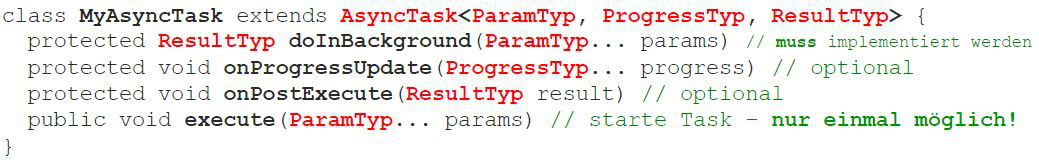
\includegraphics[width=\linewidth]{fig/asynctask}
\caption{\texttt{AsyncTask}}
\label{fig:asynctask}
\end{figure}

Bei den Java-Threads muss die \texttt{run()}-Methode vom Interface \texttt{Runnable} implementiert werden. Die Klasse welche \texttt{Runnable} implementiert hat, wird dann einer \texttt{Thread}-Klasse übergeben und mit \texttt{start()} gestartet. 